\documentclass[11pt,a4paper]{article}

\usepackage[margin=2.0cm]{geometry}
\usepackage{amsmath,amssymb}
\usepackage{graphicx}
\usepackage{booktabs}
\usepackage[hidelinks]{hyperref}
\usepackage{caption}
\usepackage{float}

\captionsetup{font=small,labelfont=bf,width=.95\textwidth}
\setlength{\parindent}{0pt}
\emergencystretch=2em

\title{DUST on the small code-carried model:\\ the dust\_schedule sweep at 512 draws per bottleneck}
\author{}
\date{2026-10-27}

\begin{document}
\maketitle
\vspace{-2.5em}

\begin{figure}[H]
\centering
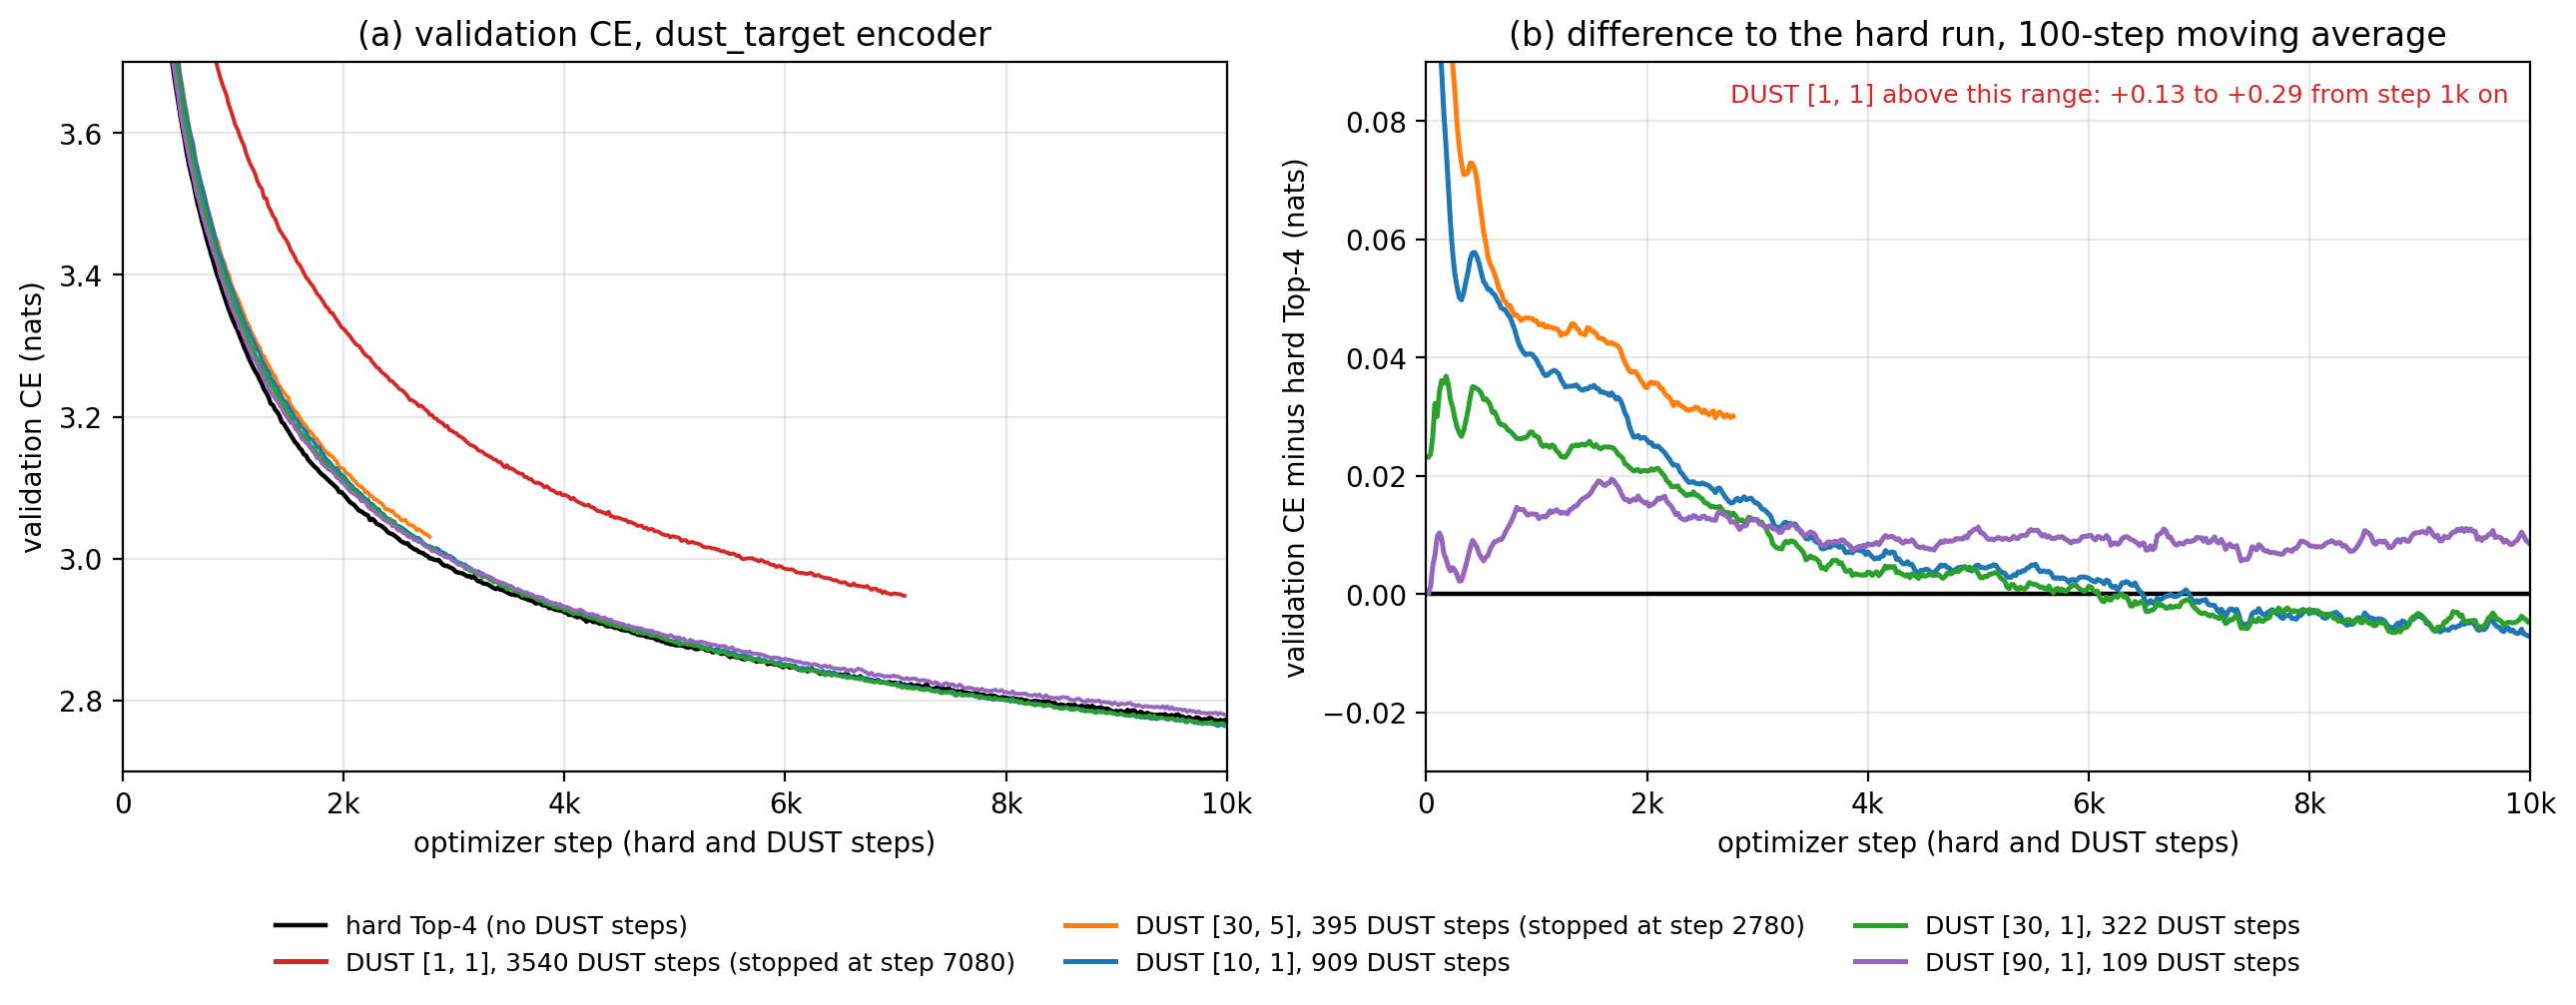
\includegraphics[width=\textwidth]{figures/small_sched_encoder.png}
\caption{\textbf{dust\_target encoder.}
Model: 4 blocks of width 128 (2 heads), a Top-4 bottleneck of $N = 512$
features at \texttt{residual\_out} of every block with the code carried
between blocks (\texttt{code\_residual}), no bottleneck post-norm,
magnitude-direction decoupling, the 8192-token BPE of TinyStories, batch
$96 \times 512$ tokens, constant learning rate $6\cdot10^{-4}$, no gradient
clipping, 10\,000 optimizer steps, seed 1337.
The black curve trains with hard Top-4 steps only.
The coloured curves interleave DUST steps by \texttt{dust\_schedule}
$[n_h, n_d]$: every period of $n_h + n_d$ optimizer steps starts with $n_h$
hard steps followed by $n_d$ DUST steps; the legend gives the number of DUST
steps up to the last plotted step.
DUST settings: 512 draws per bottleneck on the whole pool $J = N - K = 508$,
$\sigma = 0.1$ (absolute), $\gamma = 0$, a separate Adam instance for the
DUST steps at the same learning rate (\texttt{dust\_lr\_scale} 1), the
draws split over 8 GPUs.
(a) Validation CE: 40 batches of 24 windows of 512 tokens, the same windows
in every run, every 20 steps; the axis starts at 3.7 nats, so the first
$\approx 500$ steps are not shown.
(b) Validation CE minus that of the hard run at the same step, centred moving
average over 5 validations (100 steps); between neighbouring validations the
unsmoothed difference fluctuates by about 0.0015 nats.
The $[1, 1]$ run (red) lies above the range of (b).
The $[1, 1]$ and $[30, 5]$ runs were stopped by request, at steps 7096 and
2796; their last validations are at steps 7080 and 2780.
Single runs.}
\end{figure}

\begin{figure}[H]
\centering
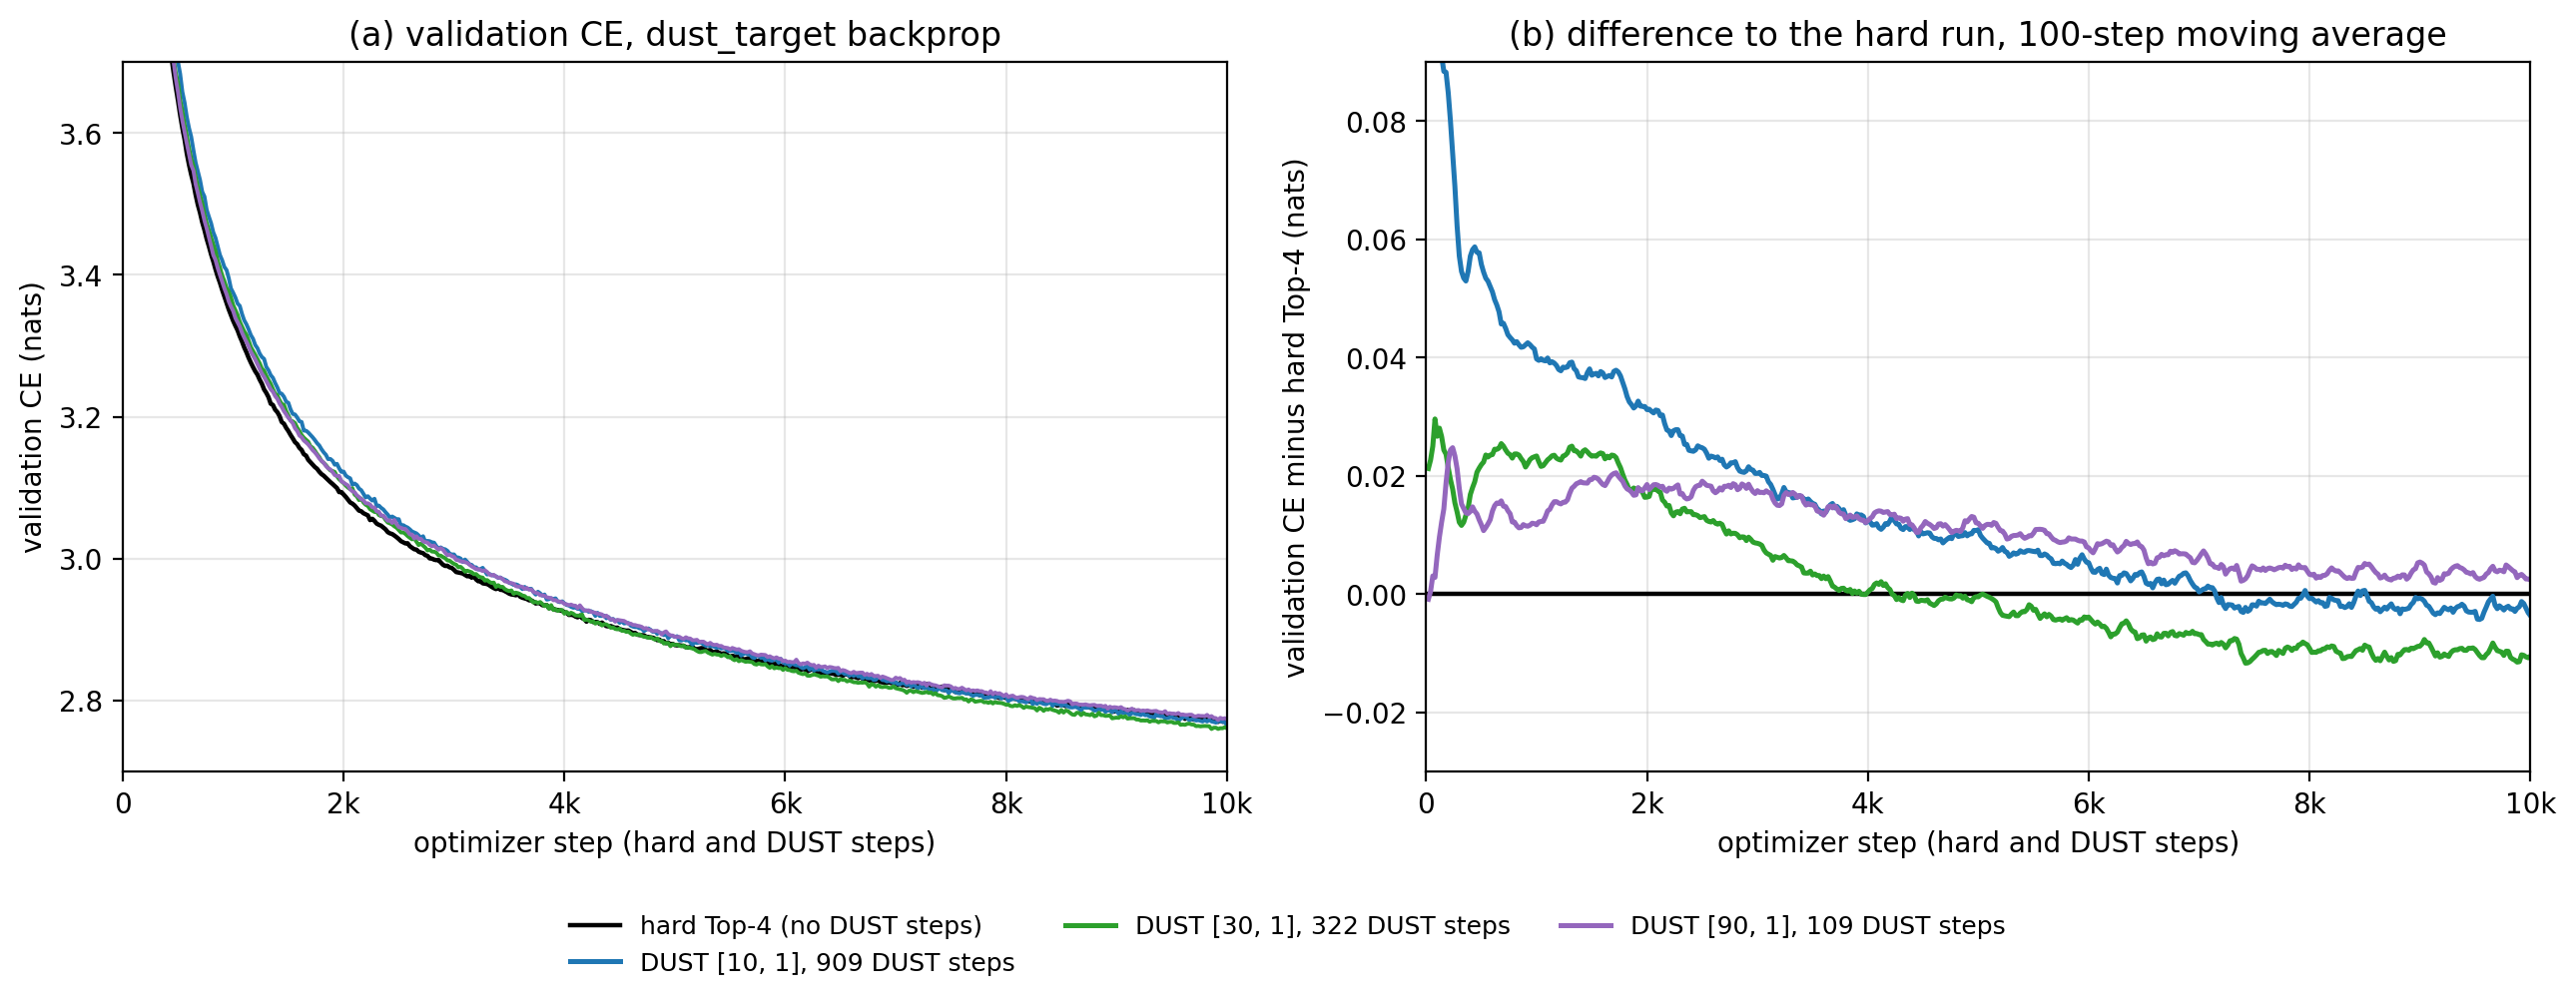
\includegraphics[width=\textwidth]{figures/small_sched_backprop.png}
\caption{\textbf{dust\_target backprop.}
As Figure~1, with the DUST estimate at every gate input backpropagated to
every parameter before that gate (\texttt{dust\_target backprop}) instead of
applied to the gate's encoder only.
No $[1, 1]$ or $[30, 5]$ run with this target.}
\end{figure}

\begin{figure}[H]
\centering
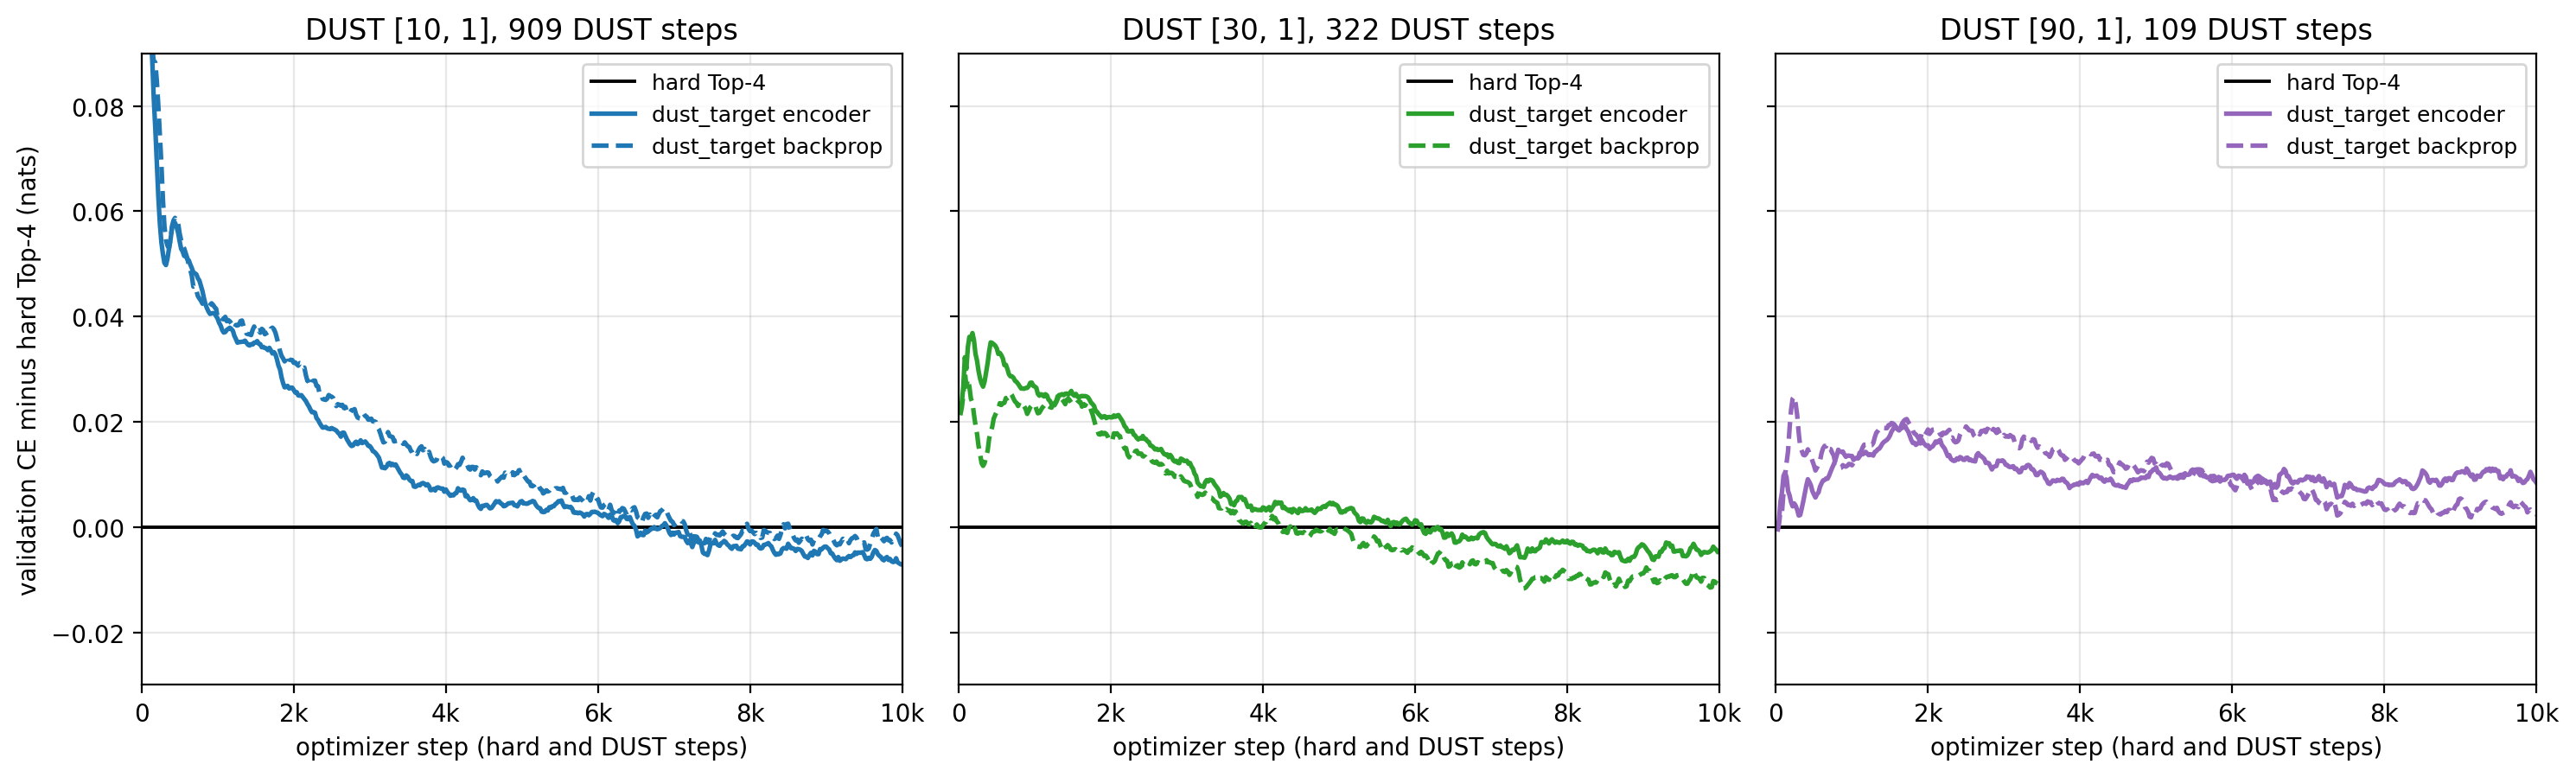
\includegraphics[width=\textwidth]{figures/small_sched_enc_vs_bp.png}
\caption{\textbf{Encoder and backprop targets per schedule.}
The curves of Figures~1b and~2b, one panel per \texttt{dust\_schedule}:
validation CE minus that of the hard run at the same step, 100-step moving
average; solid encoder, dashed backprop.}
\end{figure}

\begin{figure}[H]
\centering
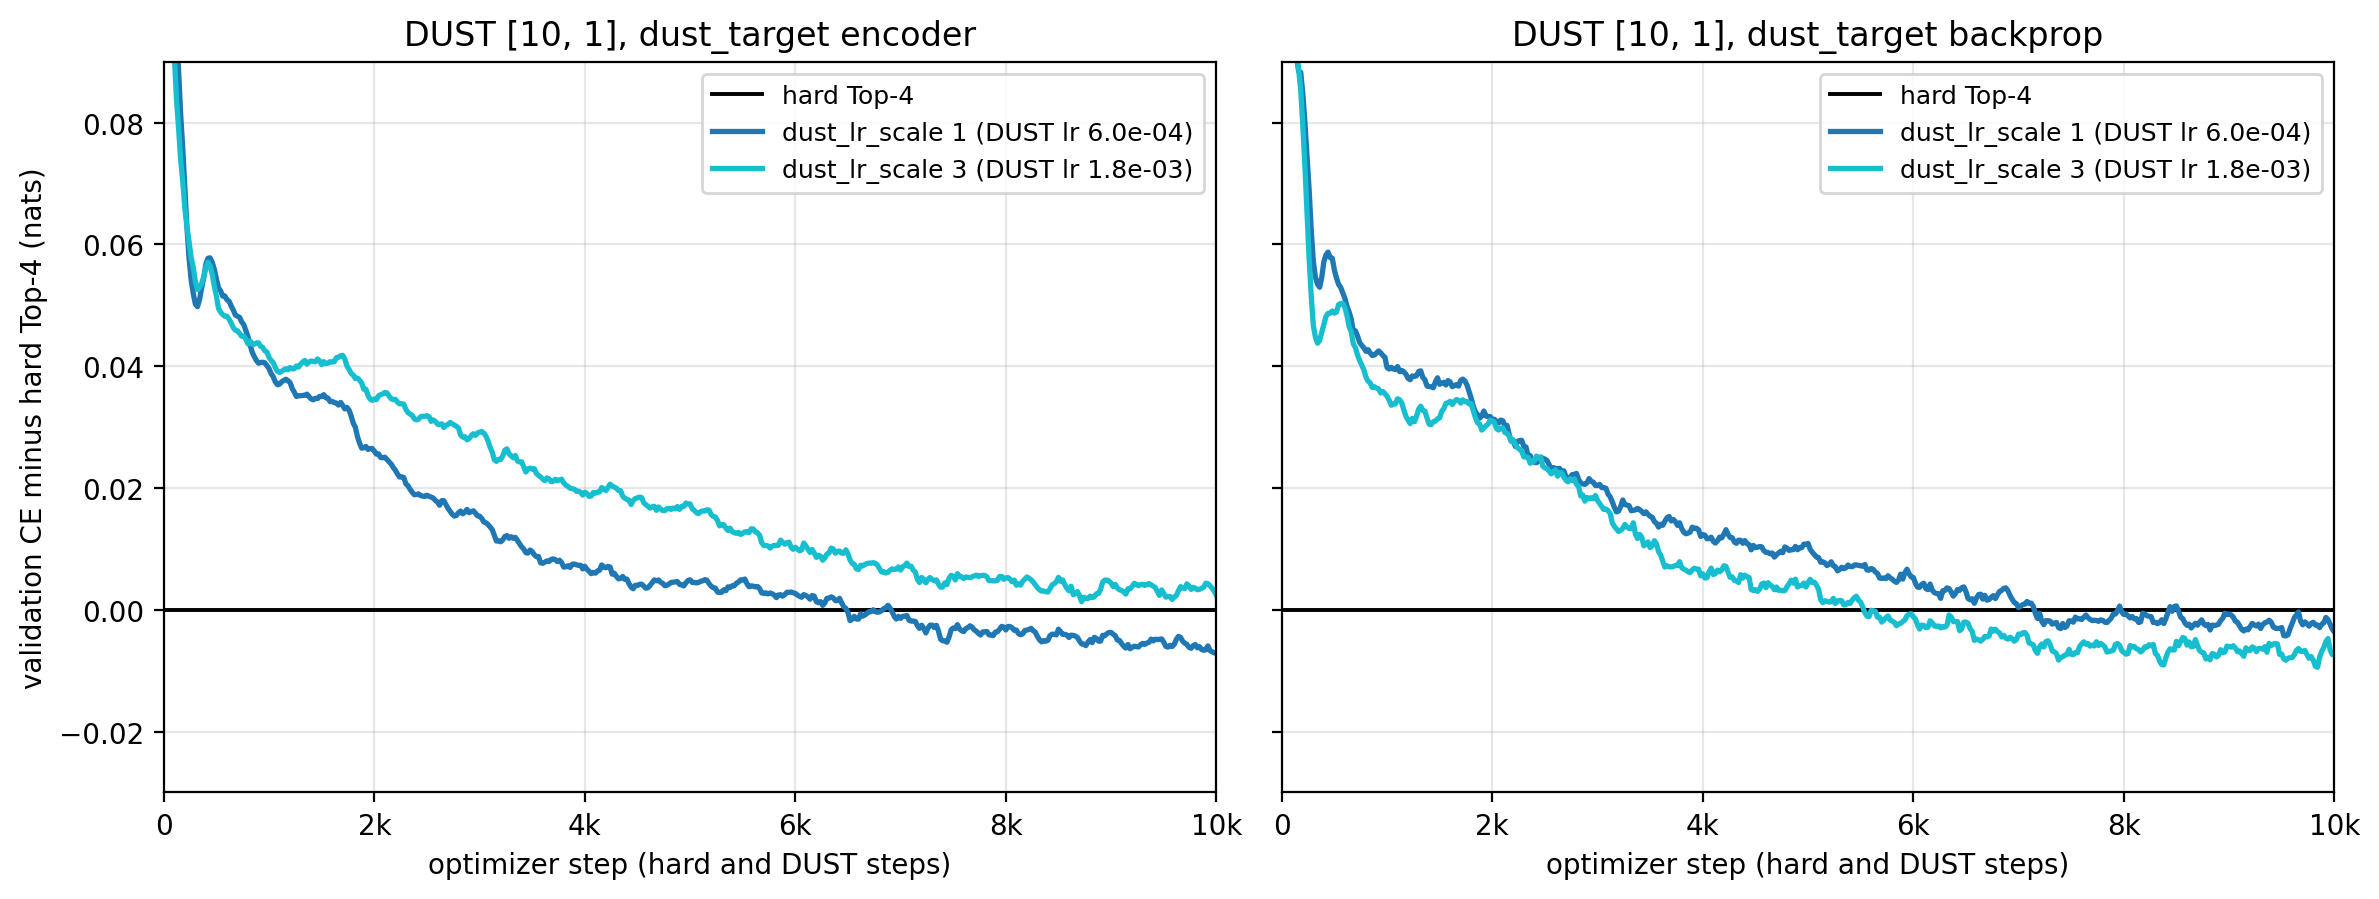
\includegraphics[width=\textwidth]{figures/small_sched_lr3.png}
\caption{\textbf{dust\_lr\_scale at $[10, 1]$.}
The learning rate of the DUST optimizer at $6\cdot10^{-4}$
(\texttt{dust\_lr\_scale} 1, the runs of Figures~1--3) and at
$1.8\cdot10^{-3}$ (\texttt{dust\_lr\_scale} 3); the hard steps use
$6\cdot10^{-4}$ in all runs.
Validation CE minus that of the hard run at the same step, 100-step moving
average; left encoder, right backprop.}
\end{figure}

\section*{Runs}

Each run is at\\
\path{gdrive:weight-sparsity/runs_warsaw/<run>/}\\
(box warsaw, 8$\times$ RTX 5090) with \path{metrics.jsonl}, \path{config.yaml},
\path{config.json}, the TensorBoard events in \path{tb/}, and a checkpoint
every 500 steps (\path{ckpt_step<N>.pt}, all kept, and \path{latest.pt});
the stopped runs carry \path{stopped.json}.  The configs are
\path{configs/small_dust/<run>.yaml}; the figures are made by
\path{scripts/plot_small_dust_sweep.py} from the \path{metrics.jsonl} files.

\begin{table}[H]
\centering
\small
\begin{tabular}{llllll}
\toprule
run & \texttt{dust\_schedule} & \texttt{dust\_target} & lr scale & steps & checkpoints \\
\midrule
\path{wa_k4_hard} & (hard only) & -- & -- & 10\,000 & 500--10\,000 \\
\path{wa_k4_dust_p512} & $[1, 1]$ & encoder & 1 & 7096$^\ast$ & 500--7000 \\
\path{wa_k4_dust_p512_h30_d5} & $[30, 5]$ & encoder & 1 & 2796$^\ast$ & 500--2500 \\
\path{wa_k4_dust_p512_h10} & $[10, 1]$ & encoder & 1 & 10\,000 & 500--10\,000 \\
\path{wa_k4_dust_p512_h30} & $[30, 1]$ & encoder & 1 & 10\,000 & 500--10\,000 \\
\path{wa_k4_dust_p512_h90} & $[90, 1]$ & encoder & 1 & 10\,000 & 500--10\,000 \\
\path{wa_k4_dust_p512_bp_h10} & $[10, 1]$ & backprop & 1 & 10\,000 & 500--10\,000 \\
\path{wa_k4_dust_p512_bp_h30} & $[30, 1]$ & backprop & 1 & 10\,000 & 500--10\,000 \\
\path{wa_k4_dust_p512_bp_h90} & $[90, 1]$ & backprop & 1 & 10\,000 & 500--10\,000 \\
\path{wa_k4_dust_p512_h10_lr3} & $[10, 1]$ & encoder & 3 & 10\,000 & 500--10\,000 \\
\path{wa_k4_dust_p512_bp_h10_lr3} & $[10, 1]$ & backprop & 3 & 10\,000 & 500--10\,000 \\
\bottomrule
\end{tabular}

\smallskip
{\small $^\ast$ stopped by request; lr scale is \texttt{dust\_lr\_scale}; a checkpoint every 500 steps.}
\end{table}

\end{document}
